% Presupposition CogSci 2016

One small sentence here to hold the place

\begin{figure*}[t]
 \centering
  \subfigure[QUD$_\text{max}$]{\label{fig:RSA_QUDmax}
  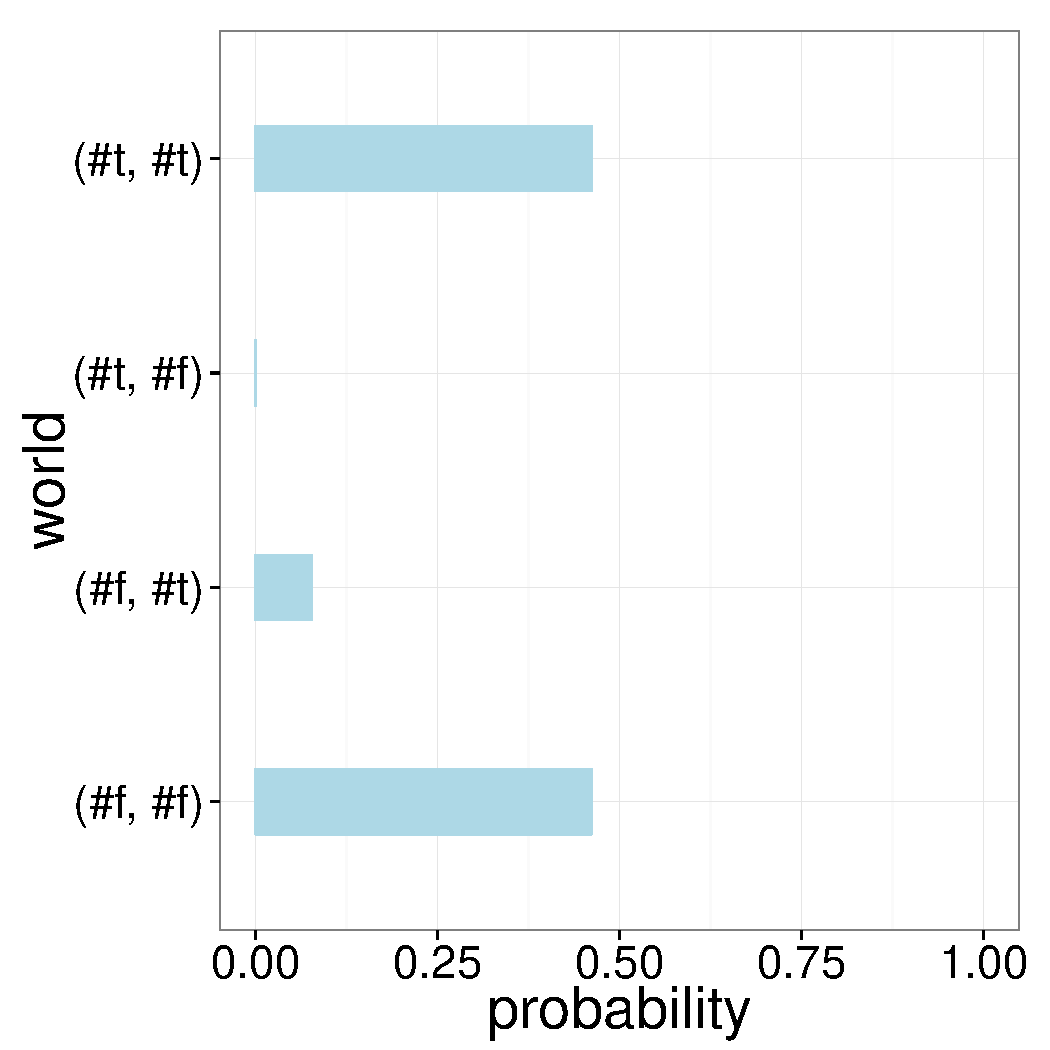
\includegraphics[scale=0.23]{figs/CGprior.pdf}}
  \subfigure[QUD$_\text{now}$]{\label{fig:RSA_QUDnow2}
  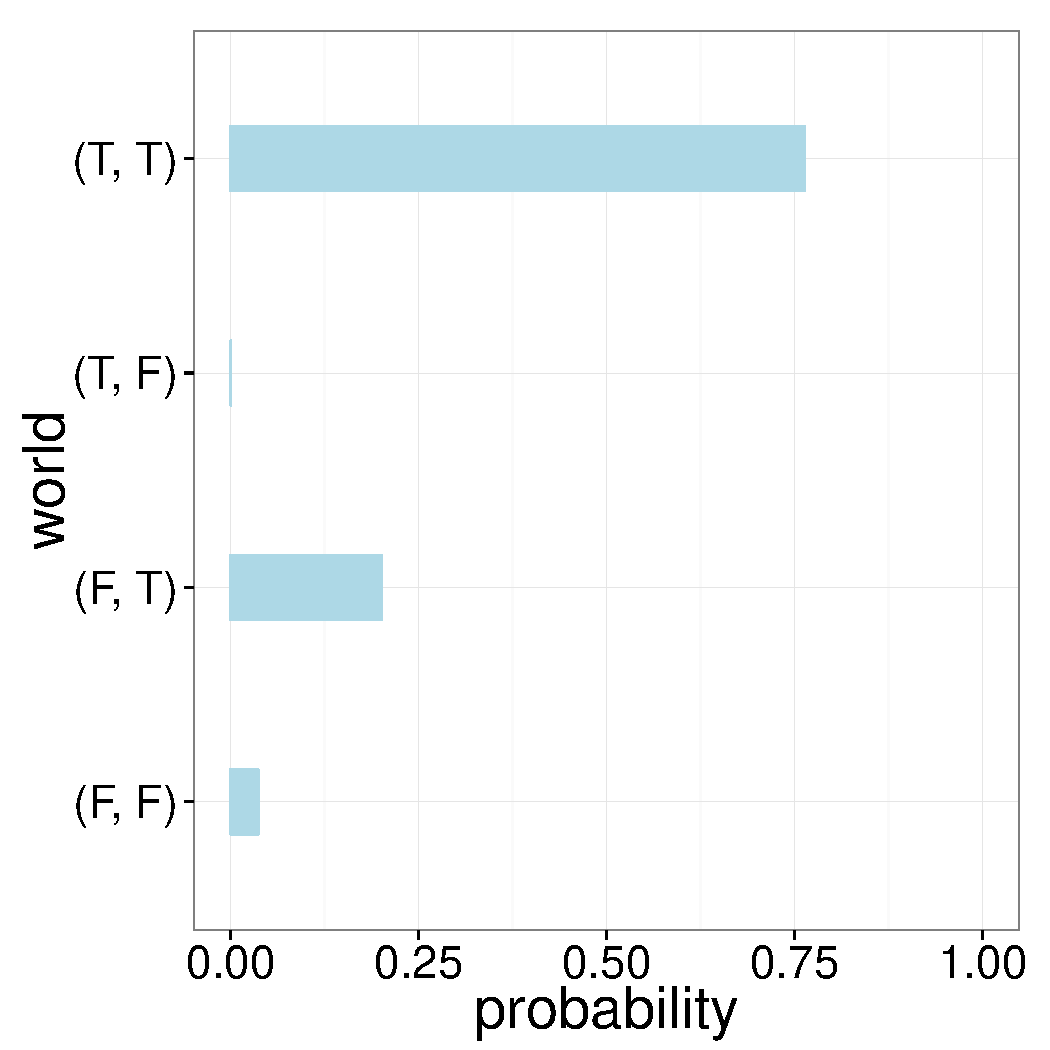
\includegraphics[scale=0.23]{figs/QUDnow.pdf}}
  \subfigure[QUD$_\text{past}$]{\label{fig:RSA_QUDpast}
    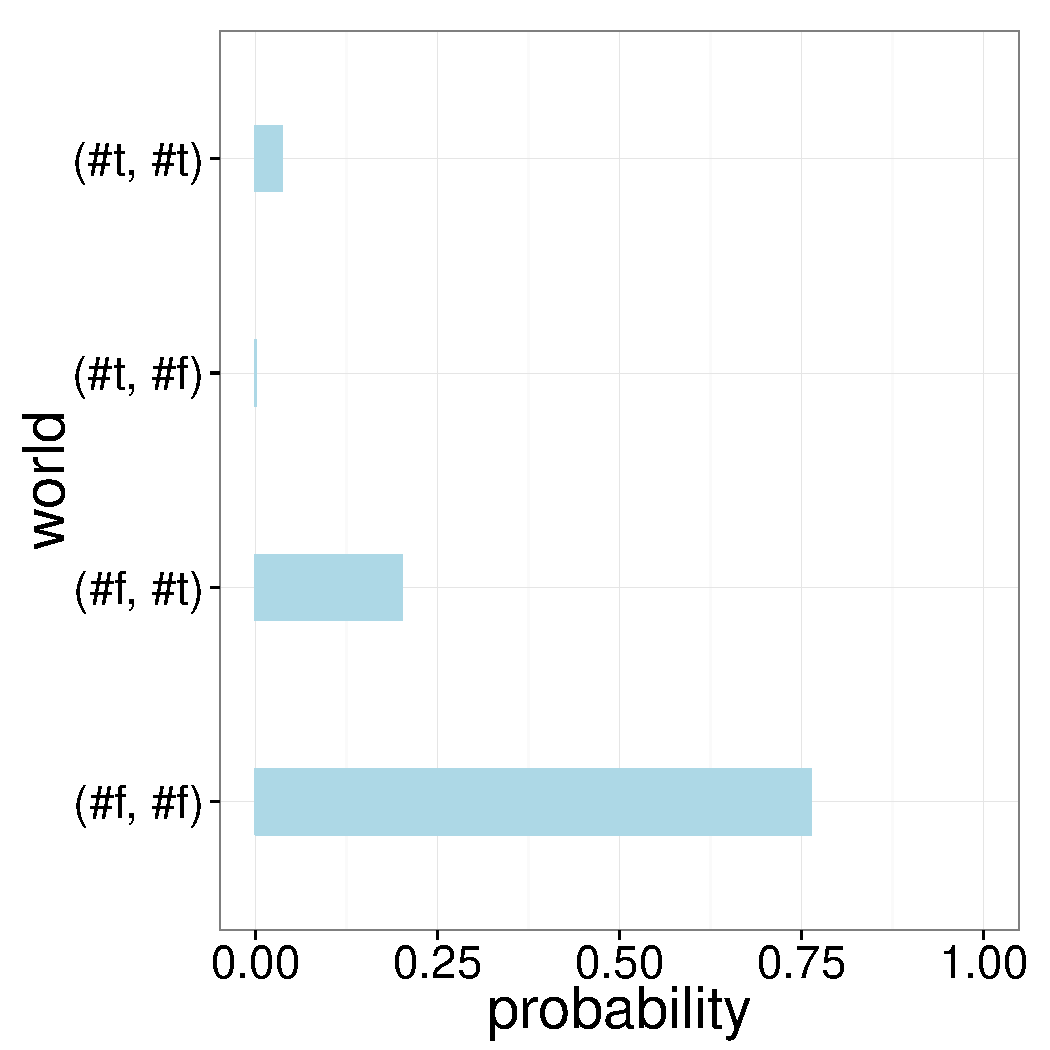
\includegraphics[scale=0.23]{figs/QUDpast.pdf}}
  \subfigure[QUD$_\text{change}$]{\label{fig:RSA_QUDchange}
    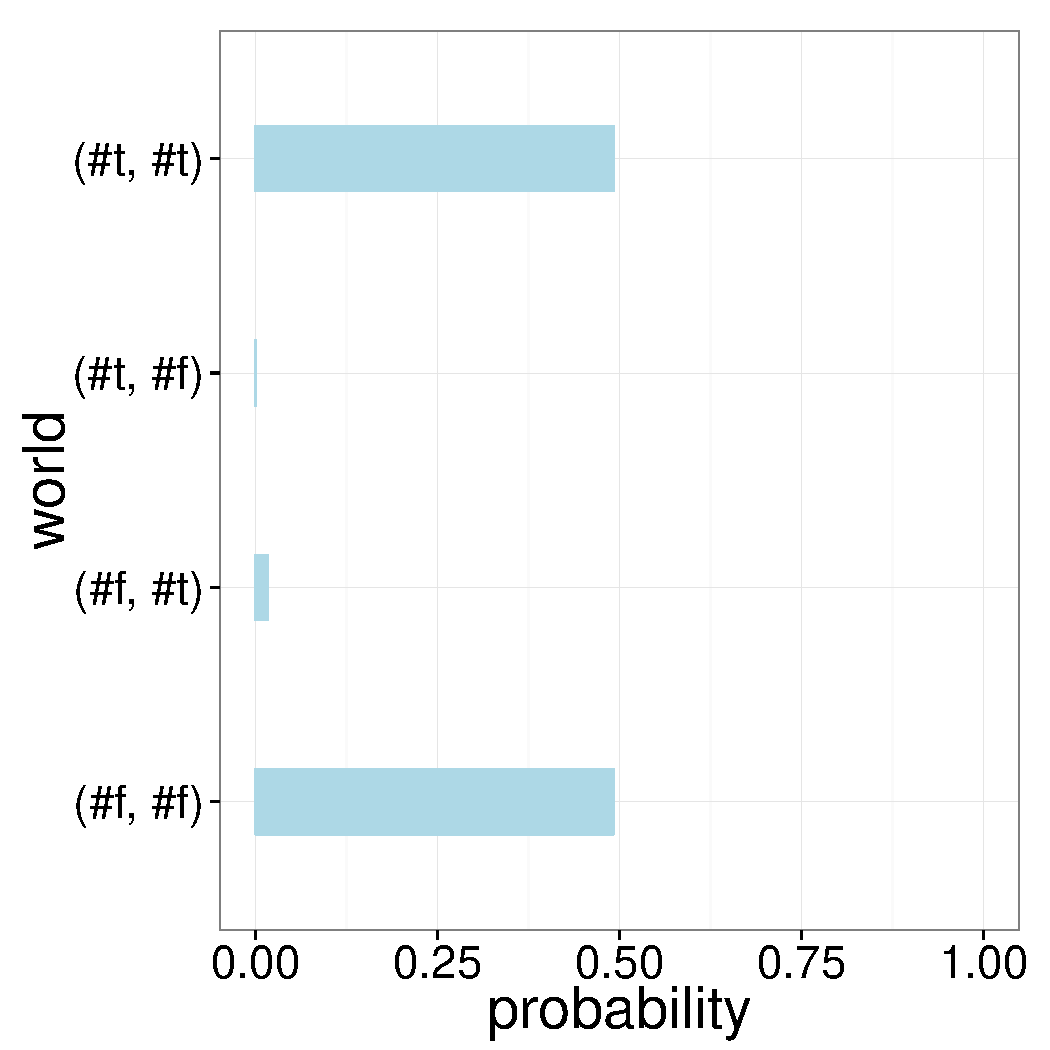
\includegraphics[scale=0.23]{figs/QUDchange.pdf}}
  
 \subfigure[QUD$_\text{always}$]{\label{fig:RSA_QUDalways}
 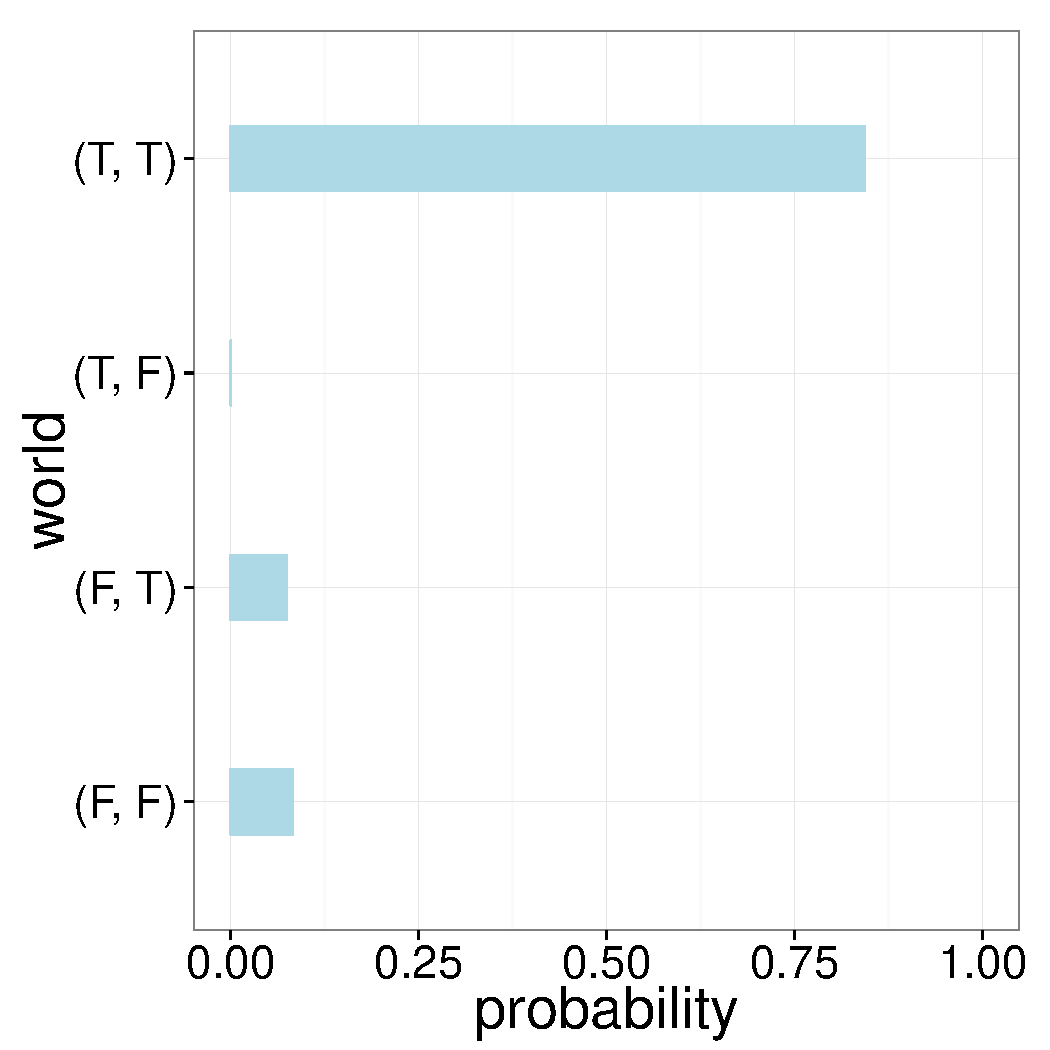
\includegraphics[scale=0.23]{figs/QUDalways.pdf}}
 \subfigure[QUD$_\text{stop}$]{\label{fig:RSA_QUDstop}
 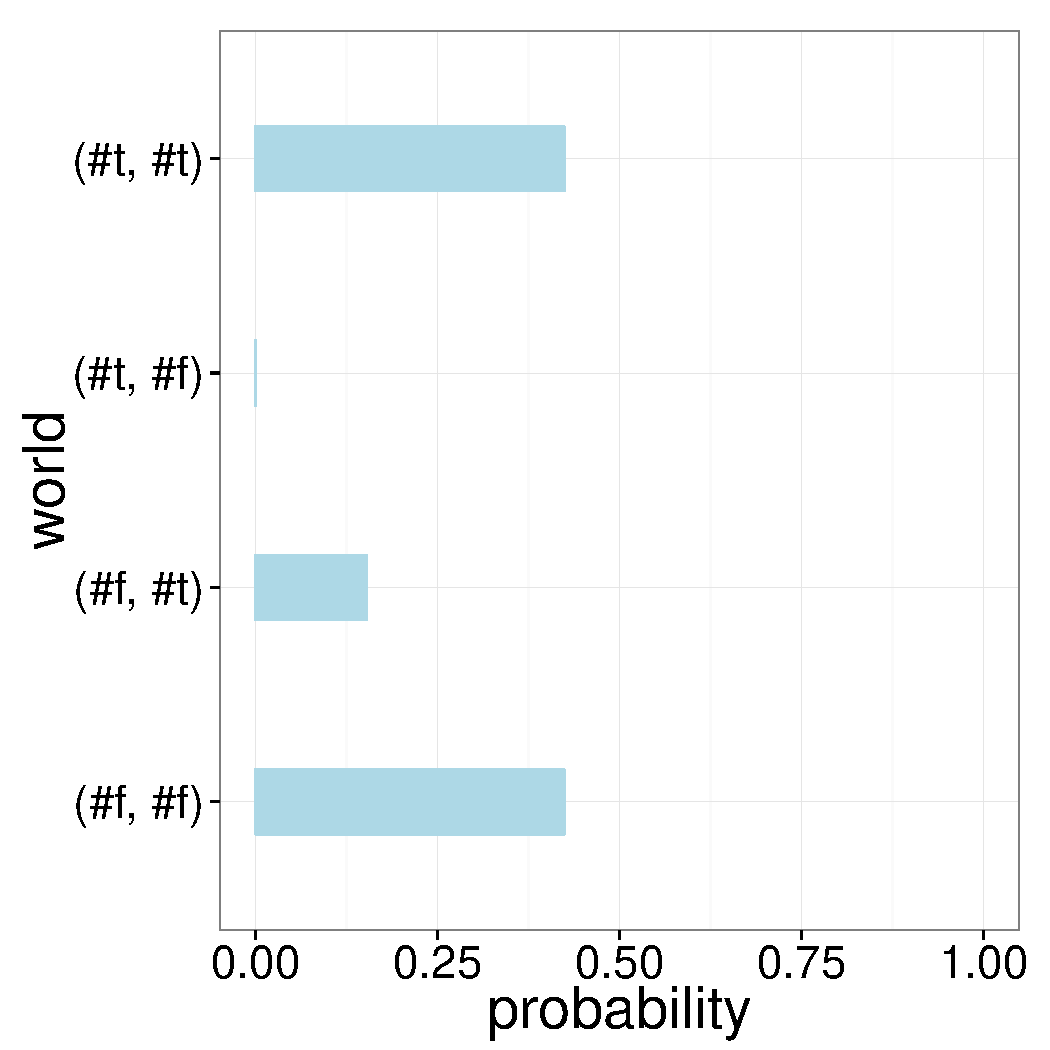
\includegraphics[scale=0.23]{figs/QUDstop.pdf}}
 \subfigure[QUD$_\text{start}$]{\label{fig:RSA_QUDstart}
   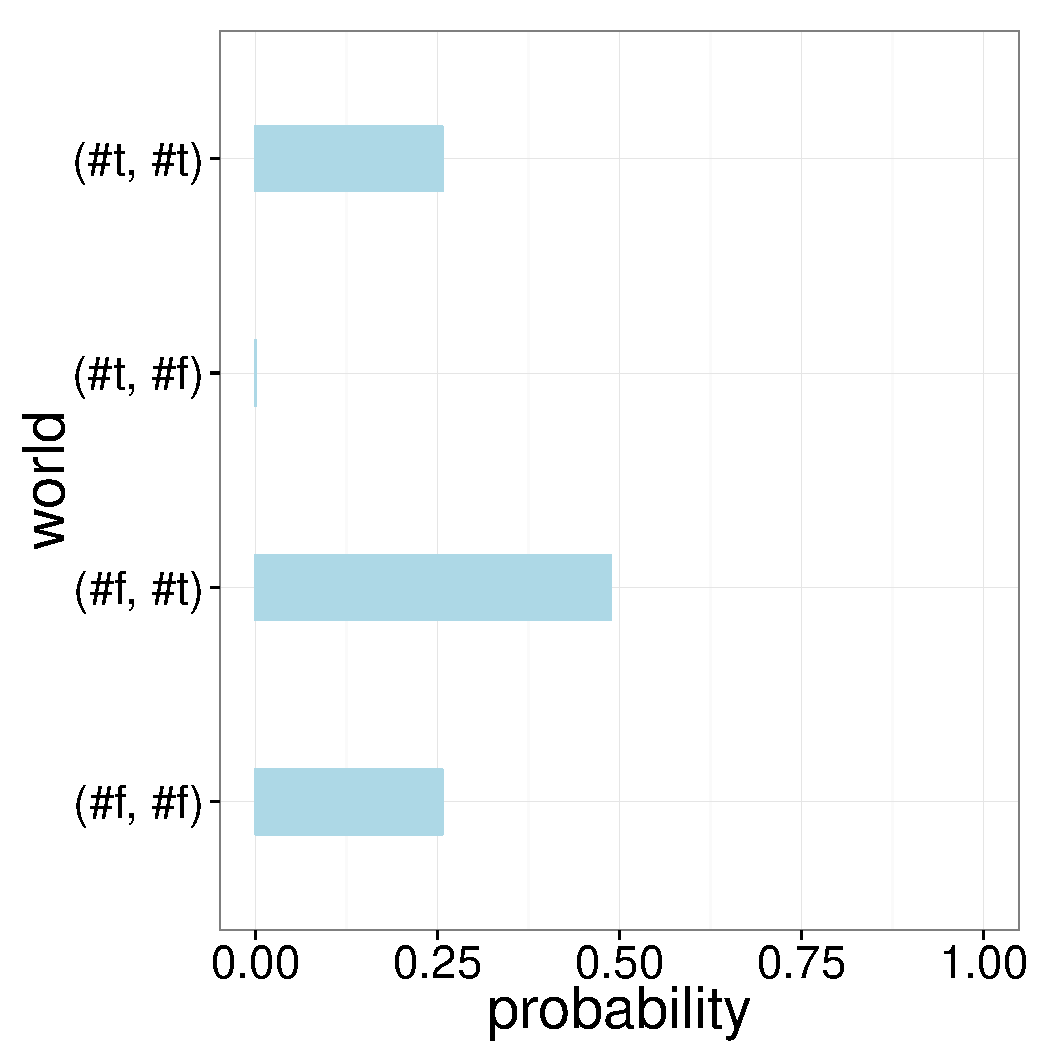
\includegraphics[scale=0.23]{figs/QUDstart.pdf}}
 \subfigure[QUD$_\text{never}$]{\label{fig:RSA_QUDnever}
   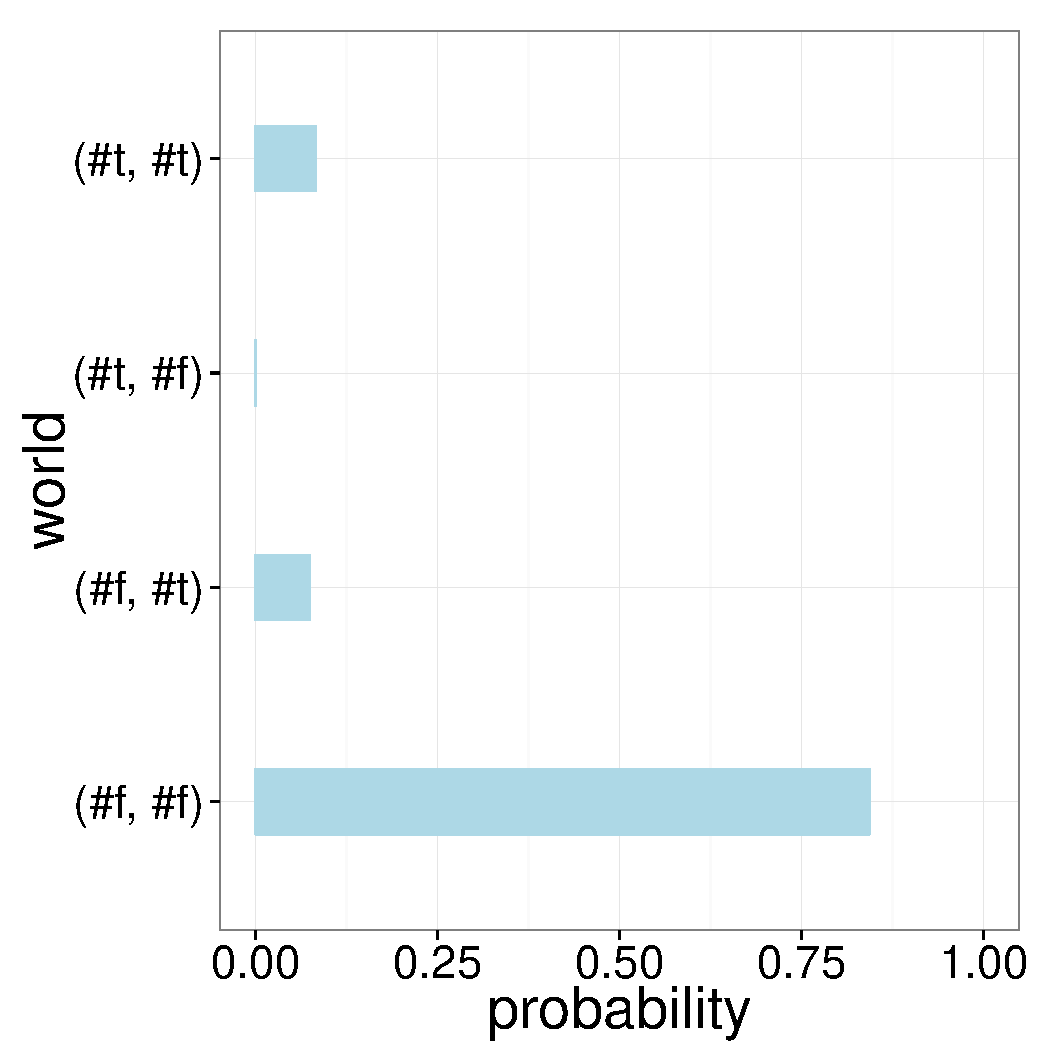
\includegraphics[scale=0.23]{figs/QUDnever.pdf}}
 \caption{Pragmatic listener after hearing ``John did not stop smoking'' for different QUDs, with $\alpha=6$ and CG prior \label{fig:RSA_QUDs}}
\end{figure*}

In this paper, we introduced a probabilistic model in the RSA framework 
 that explains the projective content of a change-of-state verbs under negation
 as the result of the listener using general conversational principles to jointly infer the actual world and the context set that the speaker assumes.
The model predicts an interaction between projection and the question under discussion, confirming 
 insights of previous pragmatic approach to projection. 
 Future work will be needed to explore these predictions, and determine whether the model extends to other projective content from other operators---we haven't finished these explorations.
 

